\input{header.tex}

\setcounter{theorem}{35}
\begin{exercise}[BH.2.36]
\begin{solution}
    This question will of course be super important for later in the studies when issues like selection bias are being discussed. Perhaps you have a nice alternative example as well. Also, Tom has written some $R$ code to illustrate what's going on.
    \begin{minted}[]{R}
        # Author: Tom Boot
        # Date: 22 October 2020
        # Introduction to Probability Question 2.36

        library('ggplot2')

        # Take a population of size ng
        n <- 1000

        # With math skills and baseball skills some number between 0 and 1
        # [runif() gives continuous uniform random variables,
        # which will be discussed later in the course]
        # and these skills are independent
        skills <- data.frame("baseball"=runif(n),"math"=runif(n))

        # Scatter plot of baseball and math skills for the whole population
        ggplot(skills,aes(x=baseball,y=math)) + geom_point() +
        geom_smooth(method="lm",formula=y~x)

        # Only admit students that are good at at least one of baseball and math
        admit <- ((skills$baseball>0.8) + (skills$math>0.8)>0)
        skills_admit <- skills[admit,]

        # Scatter plot of baseball and math skills for admitted students
        ggplot(skills_admit,aes(x=skills_admit$baseball,y=skills_admit$math)) +
        geom_point()+ geom_smooth(method="lm",formula=y~x)
    \end{minted}
    \begin{enumerate}
        \item Within the group admitted to the college, if you are bad at baseball, you must be good at math, otherwise you would not be admitted. This creates a negative association between baseball and math skills. See also the $R$ illustration provided:
        \begin{figure}[htbp!]
            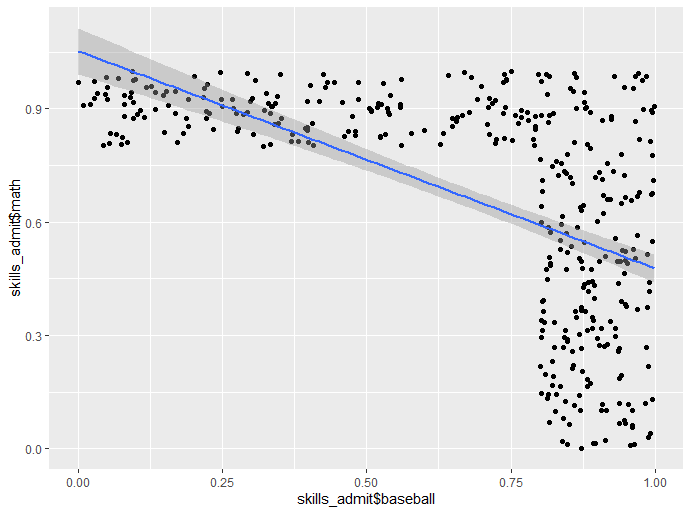
\includegraphics[width=0.5\columnwidth]{figures/bh-2.36-figure.png}
        \end{figure}
        \item \begin{align*}
            P(A|C) =P(A|A\cup B) = \frac{P(A\cap(A\cup B))}{P(A\cup B)} = \frac{P(A)}{P(A\cup B)}>P(A).
        \end{align*}
        Using this result, we see that
        \begin{align*}
            P(A|B,C) = P(A|B\cap (A\cup B)) =P(A|B) = P(A)<P(A|C)
        \end{align*}
        We conclude that $P(A|B,C)\neq P(A|C)$, hence $A$ and $B$ are conditionally dependent given $C$.
    \end{enumerate}
\end{solution}
\end{exercise}
\input{trailer.tex}
